\subsubsection{FIR Filter mit anpassbarer Grenzfrequenz}
\label{sec:LibFIRAdaptive}

Damit auf dem STM32 dynamisch ein FIR Tiefpassfilter generiert werden kann, ist die Helperlibrary \texttt{adaptive\_fir.c} im Projektordner dabei.
Die Library enthält eine Funktion, die aus für eine gewünschte Grenzfrequenz die gewünschte Anzahl Koeffizienten liefert.
Dabei wird die \textit{Windowing-Methode} \cite{FIR-Windowing}, dessen Funktionsweise hier kurz erklärt wird, verwendet.

\paragraph{Tiefpassfilter mit der Windowing Methode erzeugen}

Die Windowing Methode benutzt die Eigenschaft eines idealen Tiefpassfilters, dessen Amplitudengang einer $rect()$-Funktion (Abbildung \ref{pic:lowpass_ideal}) entspricht.
Wird $rect()$-Funktion Laplace-Transformiert, hat sie im Zeitbereich die Funktion $\frac{\sin{x}}{x}$ bzw. $sinc(x)$ - Abbildung \ref{pic:lowpass_sinc}.

\begin{figure}[H]
	\centering
	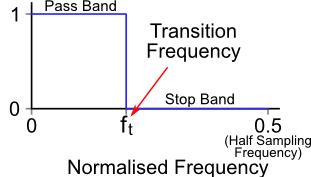
\includegraphics[width=0.4\linewidth]{lowpass_ideal}
	\caption{Amplitudengang eines idealen Tiefpassfilters mit Grenzfrequenz $f_t$ \cite{FIR-Windowing}}
	\label{pic:lowpass_ideal}
\end{figure}

\begin{figure}[H]
	\centering
	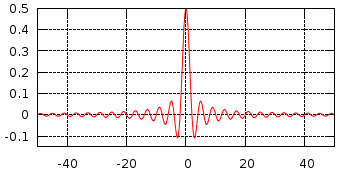
\includegraphics[width=0.4\linewidth]{lowpass_sinc}
	\caption{Die Impulsantwort eines idealen Tiefpassfilters folgt der Funktion $\frac{\sin{x}}{x}$ \cite{FIR-Windowing}}
	\label{pic:lowpass_sinc}
\end{figure}

Da die Funktion in Abbildung \ref{pic:lowpass_sinc} der Impulsantwort, und somit den Koeffizienten des Filters entspricht, lassen sich durch das Modellieren der $sinc()$-Funktion die Filterkoeffizienten berechnen.
Um das Filter zusätzlich zu verbessern, können die Koeffizienten optional mit einer der vielen Fensterfunktionen (Windows) gewichtet werden.

\paragraph{Anwendung im C-Code}

In der Helperlibrary ist eine Funktion \texttt{fir1\_win} enthalten.
Die Parameter der Funktion sind ähnlich dem MATLAB-Befehlt \texttt{fir1}.
Im unten aufgeführten Listing ist gezeigt, wie die Funktion benutzt wird, um die Koeffizienten für ein Tiefpassfilter mit der Grenzfrequenz $f_g=1.0\si{kHz}$ bei einer Samplingrate von $f_s=48.0\si{kHz}$ zu erzeugen.



\begin{lstlisting}[style=Cuvision, caption={Berechnung von 19 Koeffizienten in C}]
uint8_t num_taps = 19;
float32_t new_coeffs[num_taps];
fir1(num_taps, 1000.0f/48000.0f, new_coeffs);
\end{lstlisting}


Nachfolgend der äquivalente MATLAB Befehl mit zusätzlichen Darstellungsformen.

\begin{lstlisting}[language=matlab, caption={Berechnung von 19 Koeffizienten in MATLAB}]
num_taps = 19;
new_coeffs = fir1(num_taps-1, 1000/48000)
% Koeffizienten darstellen
stem(new_coeffs)
grid on
% Uebertragungsfunktion anzeigen
freqz(new_coeffs)
\end{lstlisting}



